\documentclass[a4paper,multicol]{article} 
\usepackage[francais]{babel}
\usepackage[utf8]{inputenc} % Required for including letters with accents
\usepackage[T1]{fontenc} % Use 8-bit encoding that has 256 glyphs
\usepackage{pythontex}
\usepackage{amsthm}
\usepackage{amsmath}
\usepackage{amssymb}
\usepackage{mathrsfs}
\usepackage{graphicx}
\usepackage{geometry}
\usepackage{stmaryrd}
\usepackage{tikz}
\usetikzlibrary{patterns}
\usetikzlibrary{patterns,math}
\usepackage{multicol}
\usepackage{hyperref}
\usepackage[cache=false]{minted}
 \definecolor{darkWhite}{rgb}{0.94,0.94,0.94}
 \usepackage[cache=false]{minted}
\definecolor{LightGray}{gray}{0.9}
\definecolor{monOrange}{rgb}{0.97,0.35,0.04}
\def \de {{\rm d}}
\usepackage{color}
\usepackage{xcolor}
\newcommand{\mybox}[1]{\fbox{$\displaystyle#1$}}
\newcommand{\myredbox}[1]{\fcolorbox{blue}{white}{$\displaystyle#1$}}
\newcommand{\mybluebox}[1]{\fcolorbox{blue}{white}{$\displaystyle#1$}}
\newcommand{\mygreenbox}[1]{\fcolorbox{green}{white}{$\displaystyle#1$}}
\newcommand{\mydoublebox}[1]{\fbox{\fbox{$\displaystyle#1$}}}
\newcommand{\myreddoublebox}[1]{\fcolorbox{red}{white}{\fcolorbox{red}{white}{$\displaystyle#1$}}}

\usepackage{geometry}
 \geometry{
 a4paper,
 total={210mm,297mm},
 left=20mm,
 right=20mm,
 top=20mm,
 bottom=20mm,
 }
%%%%%%%%%%%%%%%%%%
\usepackage{tikz}
\usetikzlibrary{patterns}
 
\newcommand*{\Rayon}{0.15}
\newcommand*{\tailleTriangle}{0.5}
\newcommand*{\largeurSol}{1}
\newcommand*{\hauteurSol}{0.4}
\pgfmathsetmacro{\basTriangle}{sin(60)*\tailleTriangle}
\newcommand*{\nbFlechesCont}{10}
\newcommand*{\rayonCouple}{0.1}
\newcommand*{\angleCouple}{110}
 
 
\tikzset{
	sol/.pic ={
		\draw[thick](-\largeurSol/2,0)--(\largeurSol/2,0);
		\fill[fill,pattern=north east lines] (-\largeurSol/2,0) rectangle++ (\largeurSol,-\hauteurSol);
	},
	mur/.pic ={
		\draw[thick](0,-\largeurSol/2)--(0,\largeurSol/2);
		\fill[fill,pattern=north east lines] (0,-\largeurSol/2) rectangle++ (\hauteurSol,\largeurSol);
	},	
	triangle/.pic ={
		\draw(0,0)--++(-60:\tailleTriangle)--++(-\tailleTriangle,0)--cycle;
		\node[anchor=south]{ \tikzpictext};
	},
	pivot/.pic ={
		\pic{triangle};
		\pic at (0,-\basTriangle){sol};
	},
	ponctuelle/.pic ={
		\pic{triangle};
		\draw(-\Rayon,-\basTriangle-\Rayon) circle(\Rayon);
		\draw(\Rayon,-\basTriangle-\Rayon) circle(\Rayon);
		\pic at(0,-\basTriangle-2*\Rayon){sol};
	},
	encastrd/.pic ={
		\pic{mur};
		\node{ \tikzpictext};		
	},
	encastrg/.pic ={
		\pic[xscale=-1]{mur};
		\node{ \tikzpictext};		
	}	
}
\newcommand{\chargecont}[4][]{% #1 (optionnel) style, #2 point de départ, #3 longueur, #4 nom de la charge
	\pgfmathsetmacro{\pas}{#3/\nbFlechesCont}
	\foreach \x in {0,\pas,...,#3}{
		\draw[latex-,#1] ([xshift=\x cm]C) --++(0,0.5);
	}
	\draw[#1]([yshift=0.5 cm]#2)--++(#3,0) node[midway,above]{#4};
}
\newcommand{\couple}[3][]{% #1 (optionnel) style, #2 point d'application, #3 nom du couple
	\draw[->,#1] (#2) +(\angleCouple:\rayonCouple) arc(\angleCouple:-\angleCouple:\rayonCouple) node[anchor=north] {$\mathcal{C}$};
}

%%%%%%%%%%%%%%%%%%%
\title{Méthode des éléments finis: TP2}
\author{Ibrahim ALAME}
\date{11/03/2024}
\begin{document}
\maketitle
\section*{Prise en Main de Cast3M}
\subsubsection*{Présentation de Cast3M}
{\em Castem2000} est un logiciel de calcul de structures par la méthode des éléments
finis et plus généralement de résolution d'équations aux dérivées partielles par la méthode des éléments finis.
Il a été développé par le Commissariat à l'Énergie Atomique (CEA).
Depuis l'été 1999, {\em Castem2000} est gratuit pour l'enseignement et la recherche, de plus le code source est ouvert aux développeurs. Il est devenu {\em Cast3M} en 2001. 
Pour débuter avec {\em Cast3M}, le point d'entrée est le site du CEA : http://www-cast3m.cea.fr/
A mettre dans vos favoris, l'utilisation de ce site est indispensable pour travailler avec {\em CAST3M}.

\subsubsection*{Installation}
La première étape de ce TP consiste à installer le code {\em Cast3M} à partir du site du CEA sur votre ordinateur (vous y avez droit en tant qu'étudiant). Nous ne détaillons pas ici les étapes de ces installations, il suffit de suivre les instructions qui vous seront données \href{http://www-cast3m.cea.fr/index.php?xml=download1}{ici}.

On pourra lancer {\em Cast3M} à partir d'une console à l'aide de la commande {\em castem22} mais je vous conseille plutôt d'utiliser l'éditeur {\em  Visual Studio} que vous pouvez installer et paramétrer de la façon suivante:
\begin{enumerate}
\item Installez {\em Visual Studio Code} pour votre platforme depuis ce lien : \href{https://code.visualstudio.com/download}{https://code.visualstudio.com/download}.
\item Une fois dans l'IDE, cliquez sur l'icon ci-dessous (1). 
\begin{center}
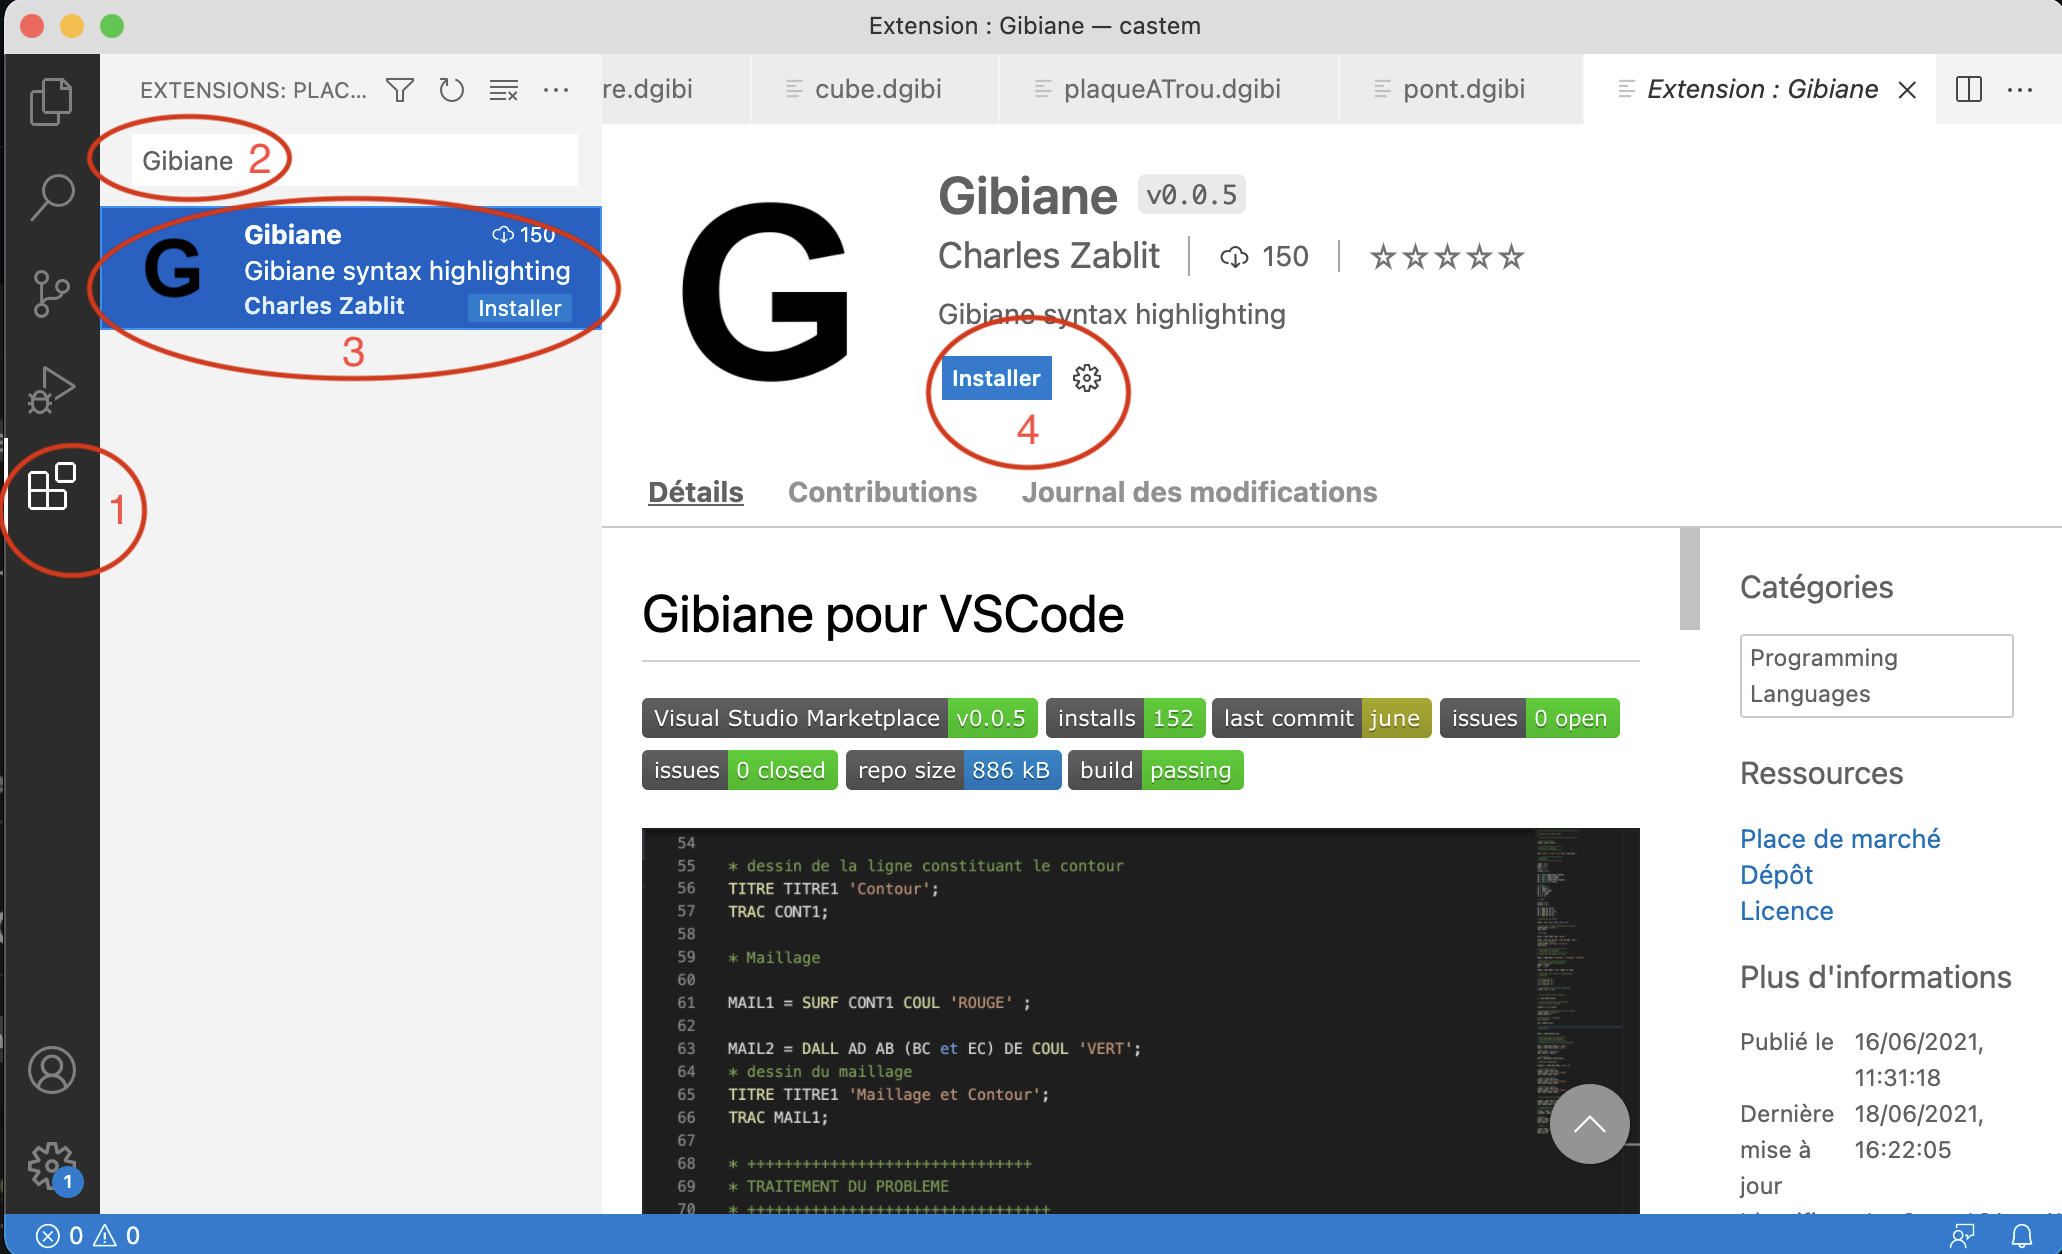
\includegraphics[scale=0.2]{installation2.png} 
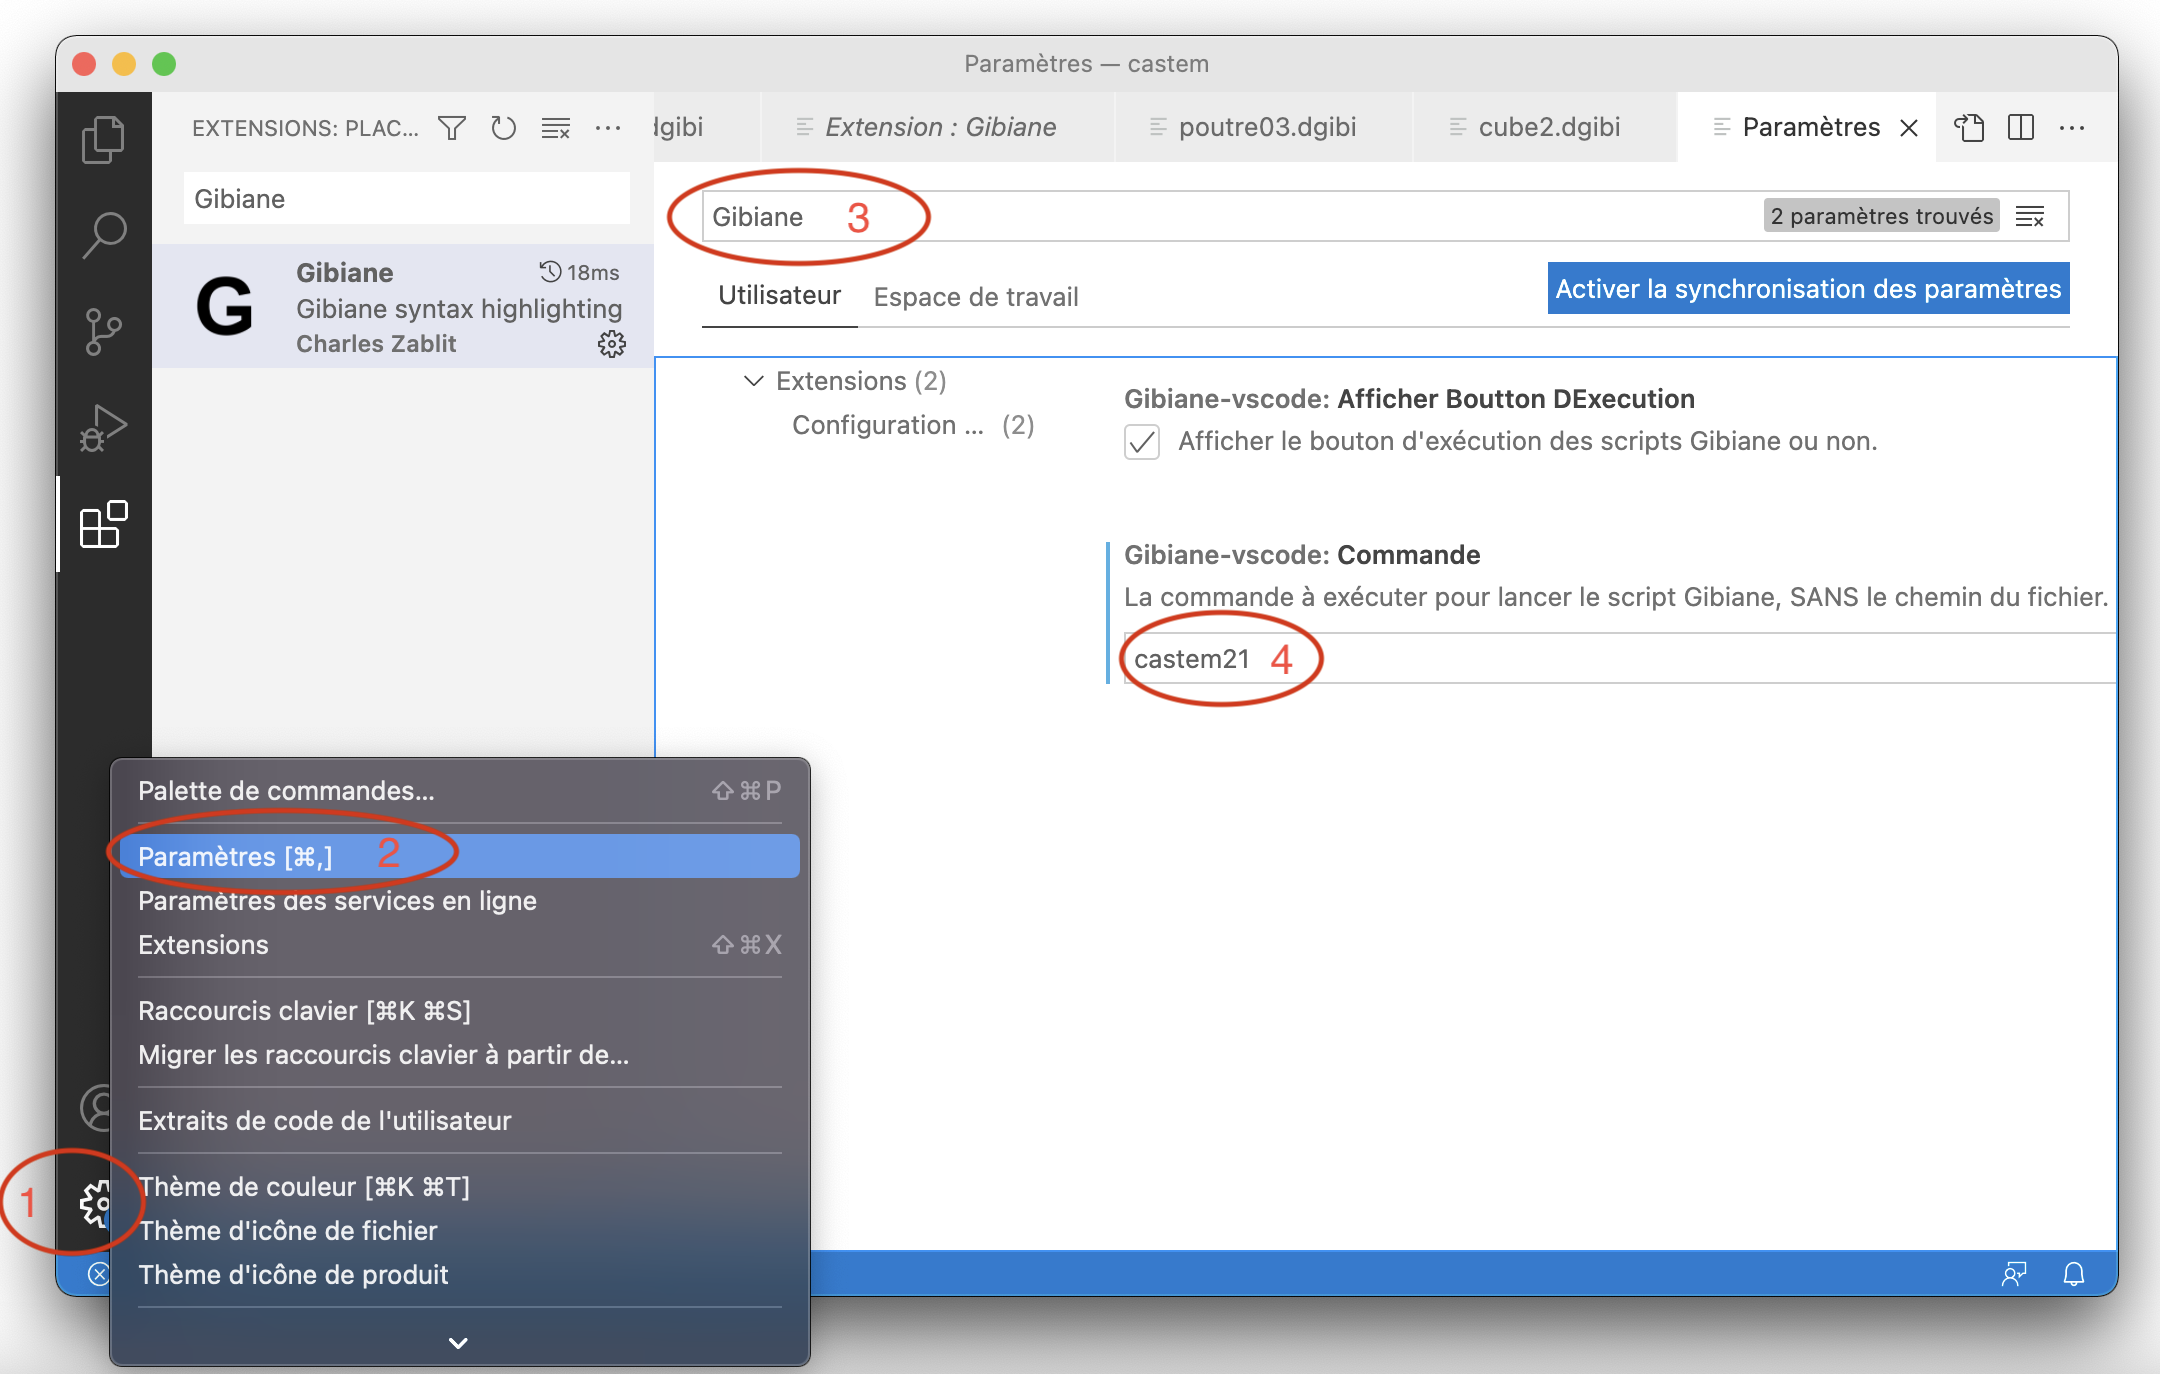
\includegraphics[scale=0.19]{configuration-2.png} 
\end{center}
\item Tapez {\tt Gibiane} dans la barre de recherche (2) et sélectionnez le premier résultat (3).
\item Cliquez sur le bouton {\tt Installer} (4).
\item Vous pouvez maintenant ouvrir votre fichier .dgibi.
\end{enumerate}
La configuration est à faire uniquement si le bouton d'exécution des scripts ne fonctionne pas!
Si c'est le cas cliquez sur la roue dentée (1) comme indiqué sur la copie d'écran à la page suivante, puis sur {\tt settings} (2), puis dans la barre de recherche (3) tapez {\tt Gibiane}. Dans le champs {\tt Gibiane-vscode}:Commande (4), rentrez le nom de la commande avec laquelle vous executez votre script habituellement. Par exemple, si vous utilisez {\tt castem22 /home/me/script.dgibi}, rentrez {\tt \color{red}castem22} uniquement. 

Cast3M possède une documentation en ligne. On peut (et on doit) la consulter pour avoir
la syntaxe d'une commande donnée. Cette documentation est au format html, on peut donc
la visualiser à l'aide d'un navigateur.
Une copie de cette documentation peut être consultée à la page
\href{http://www-cast3m.cea.fr/index.php?page=notices}{http://www-cast3m.cea.fr/index.php?page=notices} ou bien 
\href{http://www-cast3m.cea.fr/index.php?page=notices\_classees} {http://www-cast3m.cea.fr/index.php?page=notices\_classees}


\subsubsection*{Le langage de Cast3M : Gibiane}
Gibiane est le langage interprété qui permet de communiquer avec le programme. Ainsi,
le principe est d'écrire un programme en langage GIBIANE à l'aide d'un éditeur de texte
(n'importe lequel). Puis de lancer l'application castem sur le fichier créé. Il est recommandé
d'utiliser le suffixe {\tt .dgibi}.
\begin{center}
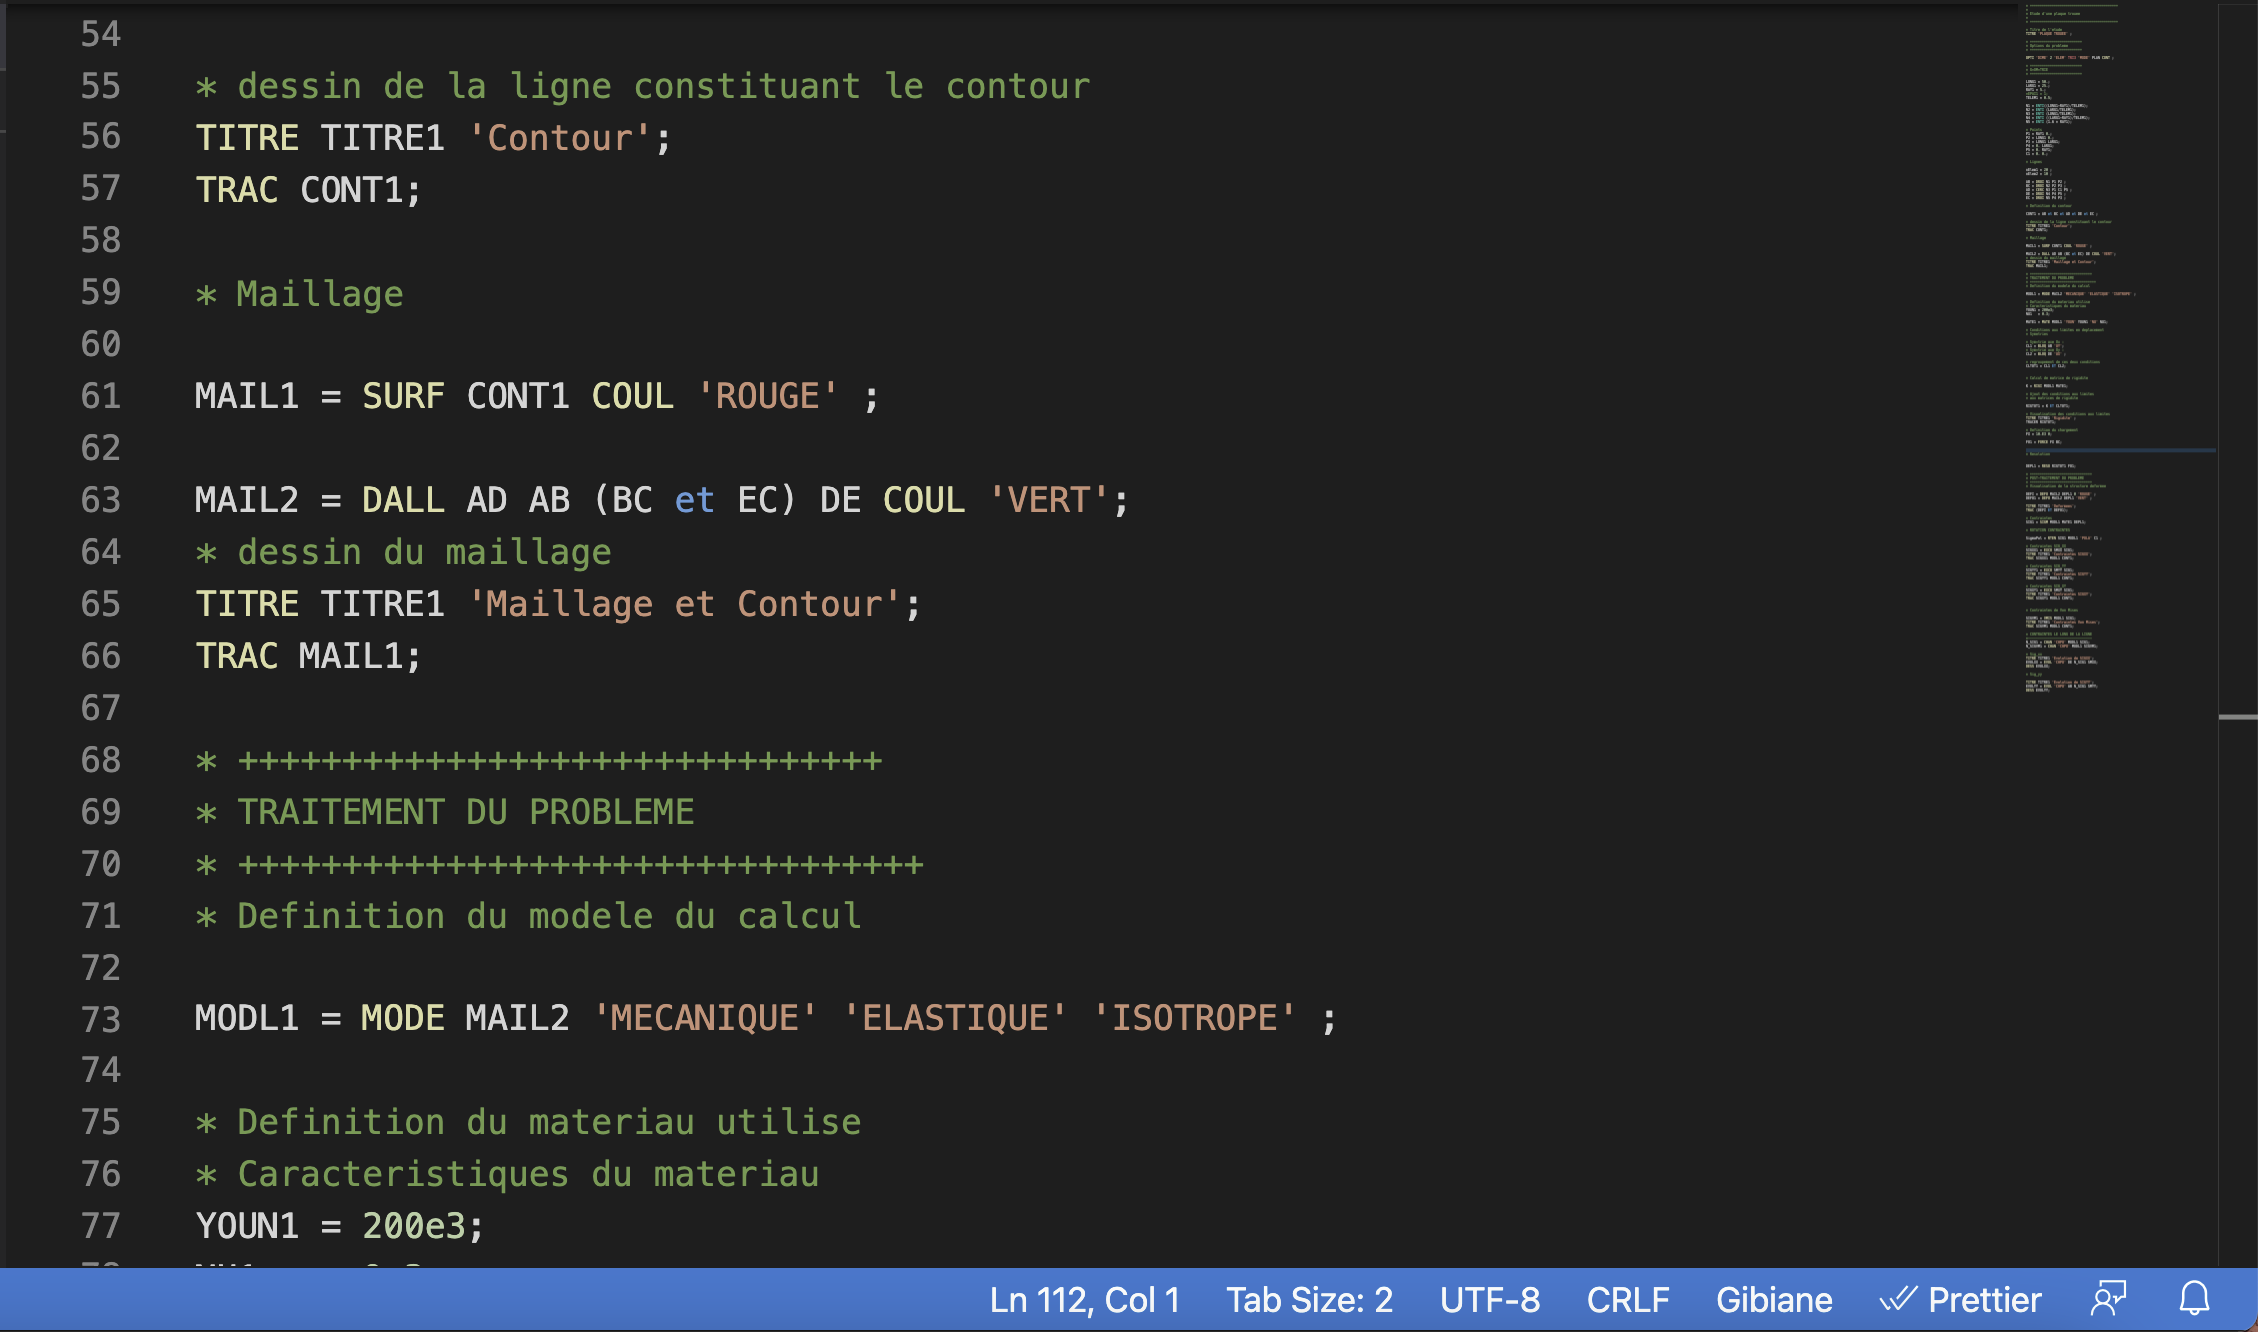
\includegraphics[scale=0.25]{example-1-1.png} 
\end{center}
La syntaxe est basée sur l'utilisation de directives, d'opérateurs et de procédures qui
s'appliquent à des opérandes. Dans le premier cas la syntaxe est :
\begin{verbatim}
DIRECTIVE OPERANDES.
\end{verbatim}
Par exemple dans
\begin{verbatim}
TRACE MAILLAGE ;
\end{verbatim}
{\tt TRACE} est la directive de traçage et {\tt MAILLAGE} est l'opérande que l'on veut visualiser. Dans
un second cas, la syntaxe est :
\begin{verbatim}
RESULTATS = OPERATEUR OPERANDES;
\end{verbatim}
Par exemple dans
\begin{verbatim}
LIGNE = DROITE P1 P2 ;
\end{verbatim}
{\tt LIGNE} sera l'objet construit en reliant {\tt P1} à {\tt P2} par une droite. {\tt DROITE} est l'opérateur qui s'applique sur les opérandes {\tt P1} et {\tt P2} et le résultat s'appelle {\tt LIGNE}. La procédure peut utiliser,
suivant sa définition, l'une ou l'autre des syntaxes. Il convient de compléter ce paragraphe en
précisant quelques règles syntaxiques de GIBIANE :
\begin{itemize}
\item Le point-virgule termine une instruction.
\item  Gibiane ne fait pas a priori de distinction entre Majuscule ou en minuscule. 
\item  Une ligne peut contenir plusieurs instructions (séparées par des points-virgules).
\item  Les lignes de commentaire sont précisées par un astérisque dans la première colonne.
\item  Les opérateurs et les directives sont définis par leurs 4 premiers caractères mais on
peut en donner plus s'il n'y a pas de confusions possibles (ex : {\tt TRAC, TRACE, TRACER}).
Il est conseillé d'utiliser un mot lisible :
{\tt TRACER} plutôt que {\tt TRAC} et {\tt DROITE} plutôt que {\tt DROI}.
\item  L'instruction est interprétée de gauche à droite, et les opérateurs sont exécutés dès
qu'ils sont lus. Ainsi {\tt 1+2*3=9} ( !) . Pour retrouver l'ordre de priorité mathématique,
il convient d'ajouter des parenthèses : {\tt 1+(2*3)=7}.
\item  La longueur du nom attribué à un objet ne doit pas dépasser 8 caractères.
Il est conseillé d'éviter d'attribuer à un objet le nom d'un opérateur existant, car ce dernier
serait alors écrasé. Pour cela on peut conseiller de ne pas donner des noms de 4 caractères et
de mettre un nombre en fin de nom (il n'y a qu'un opérateur ayant un nombre en fin de nom c'est {\tt CER3}) ou de protéger les opérateurs et directives en utilisant les côtes (ex : {\tt ‘DROI'}).
\end{itemize}
\subsubsection*{Système d'unités}
{\tt Castem} ne dispose d'aucun système particulier d'unité de mesure. 
Seule la mesure des angles doit être dans tous les cas exprimée en degrés pour la géométrie
alors que  les résultats obtenus sont en radians.
\subsubsection*{Éléments finis par Cast3M}
Tout problème d'éléments finis peut être construit de la manière suivante :
\begin{enumerate}
\item   Description de la géométrie, maillage. Choix du support géométrique.
\item   Choix du type d'éléments finis et du modèle de comportement.
\item   Donnée des caractéristiques du matériau et des caractéristiques géométriques supplémentaires.
\item   Donnée des conditions aux limites.
\item   Donnée du chargement.
\item   Résolution du système.
\item   Post-traitement des résultats.
\end{enumerate}


\subsection*{Génération de Maillage}
L'objet du maillage est de discrétiser géométriquement le domaine d'analyse de manière
à pouvoir ultérieurement associer une formulation éléments finis au support géométrique.
Concrètement cette discrétisation s'effectue par la création d'objets de type maillage (points,
lignes, surfaces, volumes) à l'aide des opérateurs géométriques. La technique à suivre est
presque toujours la même :
\begin{enumerate}
\item  construction des points
\item   construction des lignes à partir des points
\item   construction des surfaces à partir des lignes
\item   construction des volumes à partir des surfaces
\end{enumerate}
%\newpage
\subsubsection*{Maillage Simple}
Dans un premier exemple, nous allons mailler un cube de côté 10 m (l'unité en mètre est
ici indiquée pour fixer les idée, rappelons qu'il n'y a pas de système d'unité sur Castem).

\begin{multicols}{2}
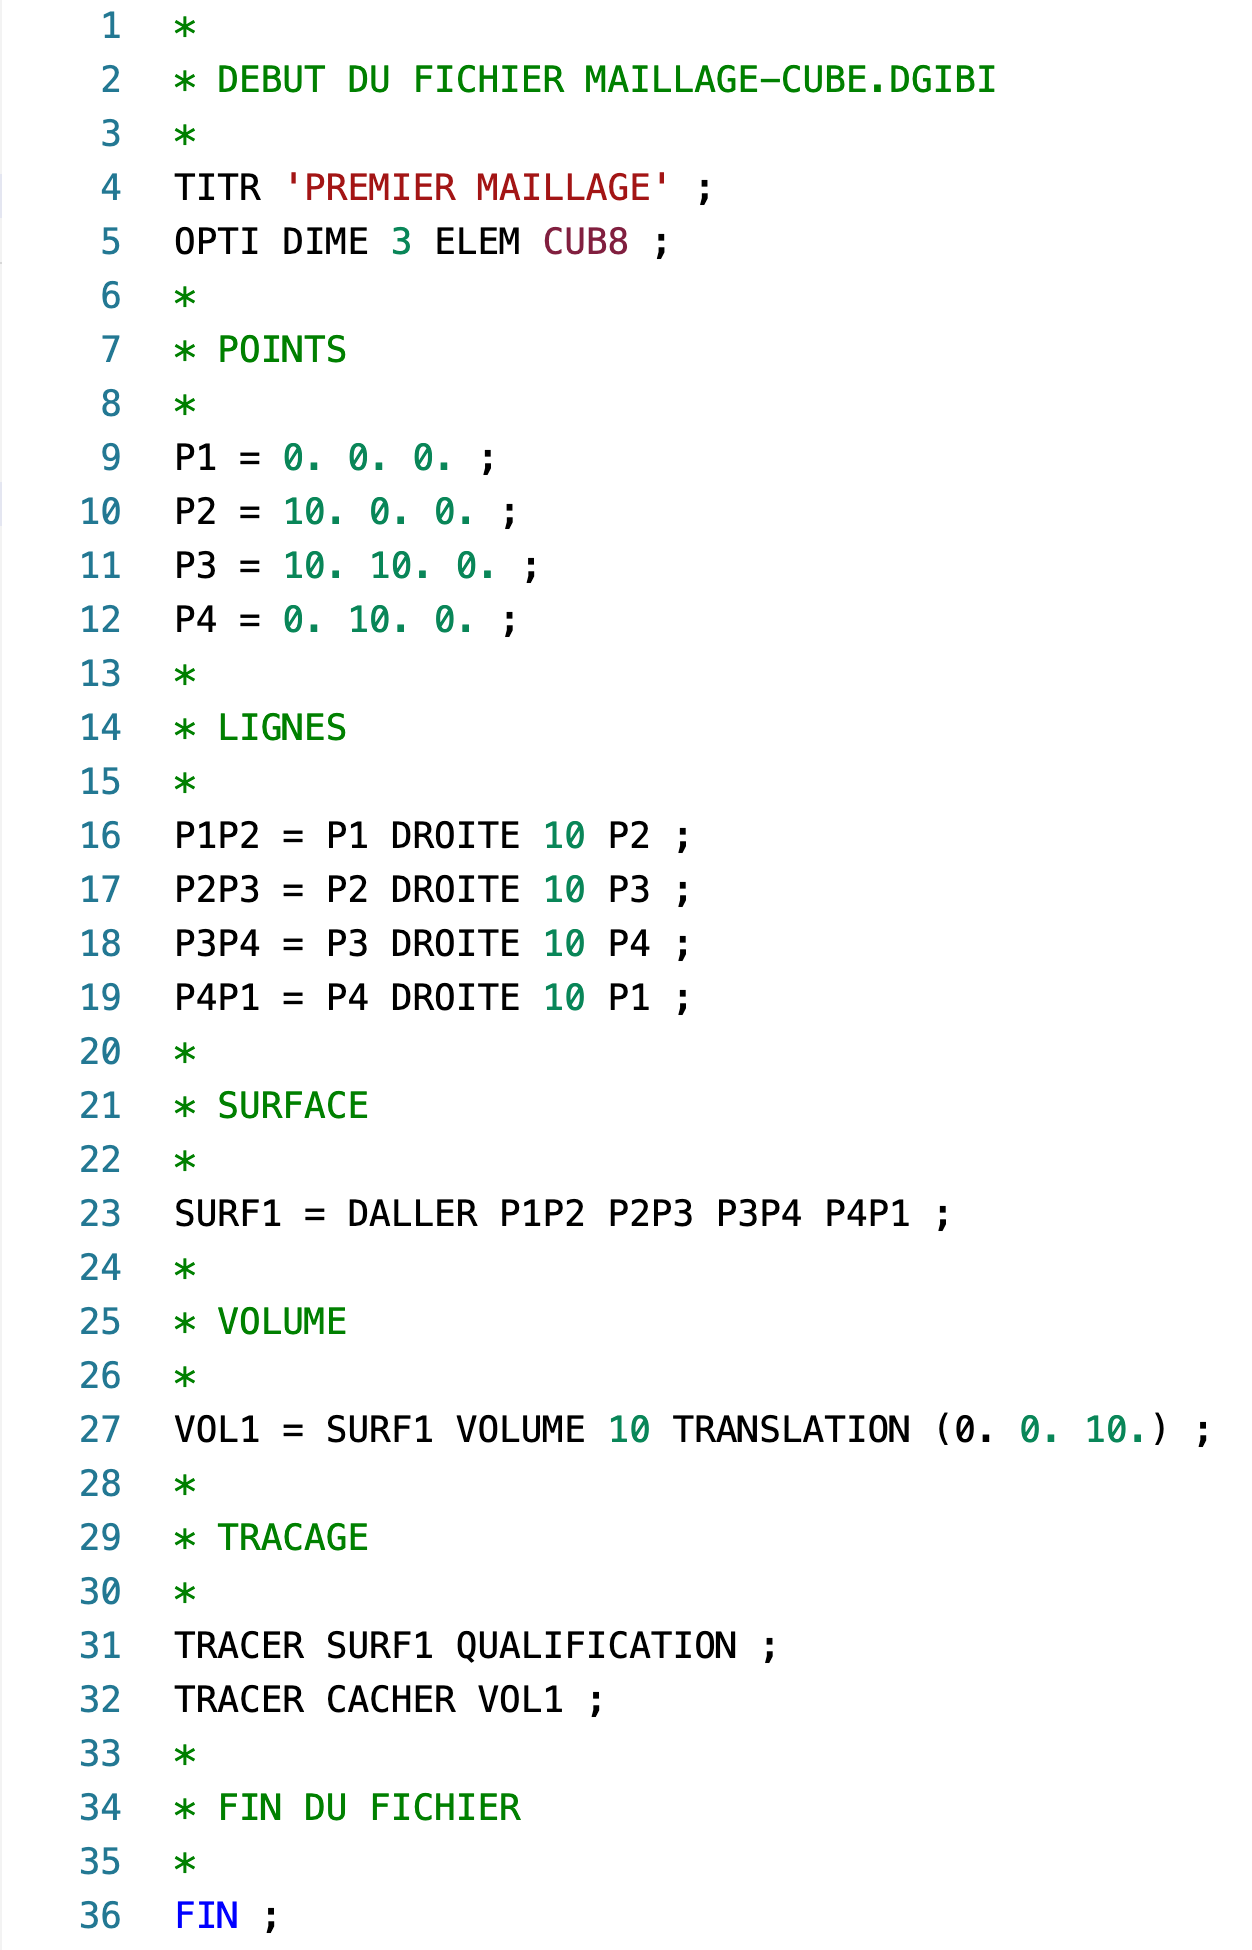
\includegraphics[scale=0.25]{pgm01Cube.png} 
\footnotesize
\begin{itemize}
\item La directive OPTI(ON) permet de déclarer les principaux paramètres du programme, par
exemple la dimension de l'espace, le type d'éléments géométriques utilisé....  
\item Le point est construit en associant à son nom, ses coordonnées.
\item L'opérateur DROI(TE) permet de construire une ligne droite à partir de ses deux points extrêmes. Ces lignes créées sont orientées et automatiquement subdivisées en un certain nombre de segments que
l'on pourra spécifier. Ici on a spécifié 10 segments entre deux points. 
\item L'opérateur DALL(ER) permet de construire une surface délimitée par 4 côtés ayant deux à deux le même nombre de points et formant une ligne fermée. 
\item L'opérateur VOLU(ME) permet de construire des volumes par translation de surface suivant un vecteur avec l'option TRAN(LATION).
\item La directive TRAC(ER) trace un objet de type maillage (ici la surface de base). L'option QUAL(IFICATION) permet d'afficher les noms des objets visualisés à l'écran.
\end{itemize}


\end{multicols}


\section*{Premier calcul mécanique linéaire}
3.1 Objectif du calcul
Le but de ce calcul est de voir sur un exemple très simple l'enchaînement des étapes nécessaires à un calcul par éléments finis par CASTEM. Pour cela on veut calculer la déformée d'une poutre encastrée à une extrémité et subissant une force fléchissant à l'autre extrémité.
Les données du problème sont :

longueur: $L=1$m, section: $ S = 1.392\times 10^{-4} m^2$, masse volumique: $\rho=7800kg/m^3$, 

inertie suivant $y$ et $z$: $I_{yy} = I_{zz} =  2.673\times 10^{-4} m^4$,
inertie de torsion:  $I_T = 1.0\times 10^{10}$, 

force appliquée: $F = 10$N , module d'Young: $E = 210000$MPa, 

\begin{multicols}{2}
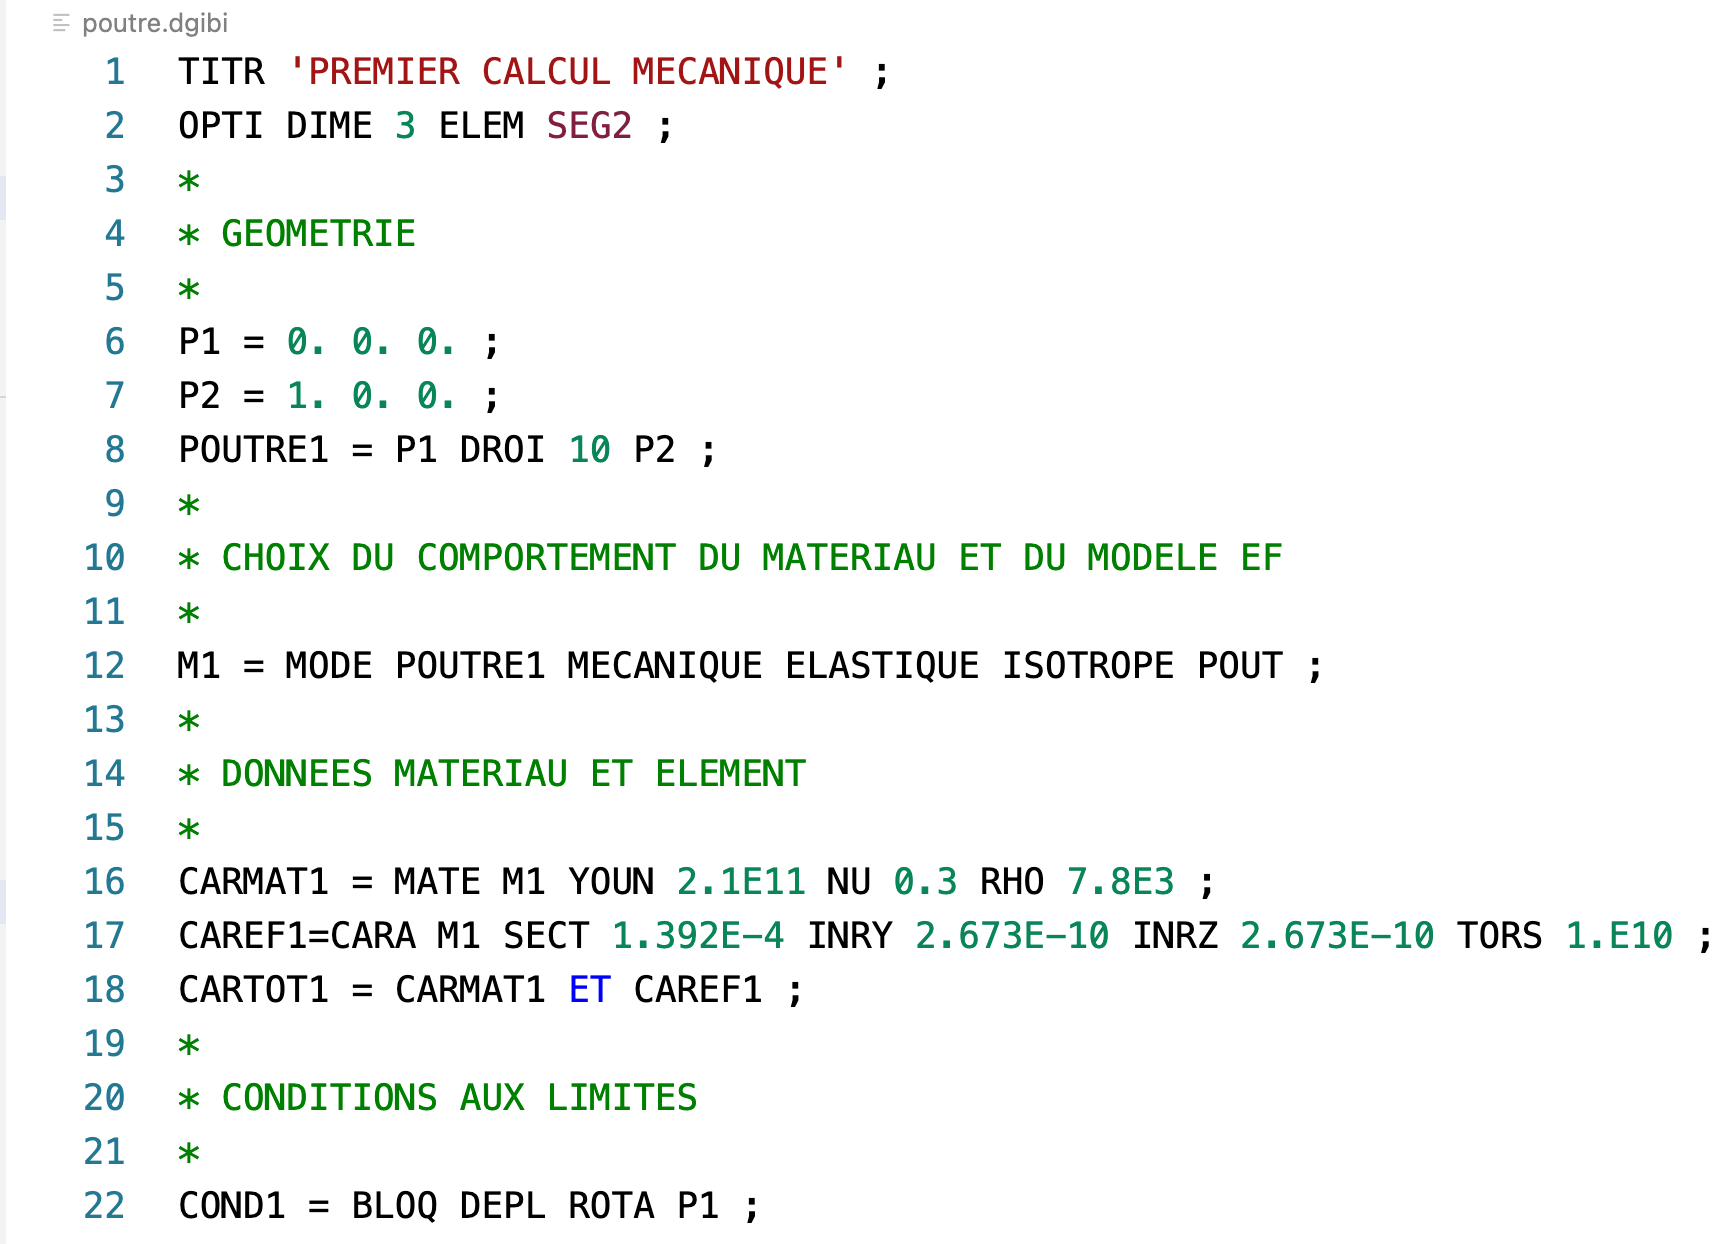
\includegraphics[scale=0.21]{poutre11.png} 
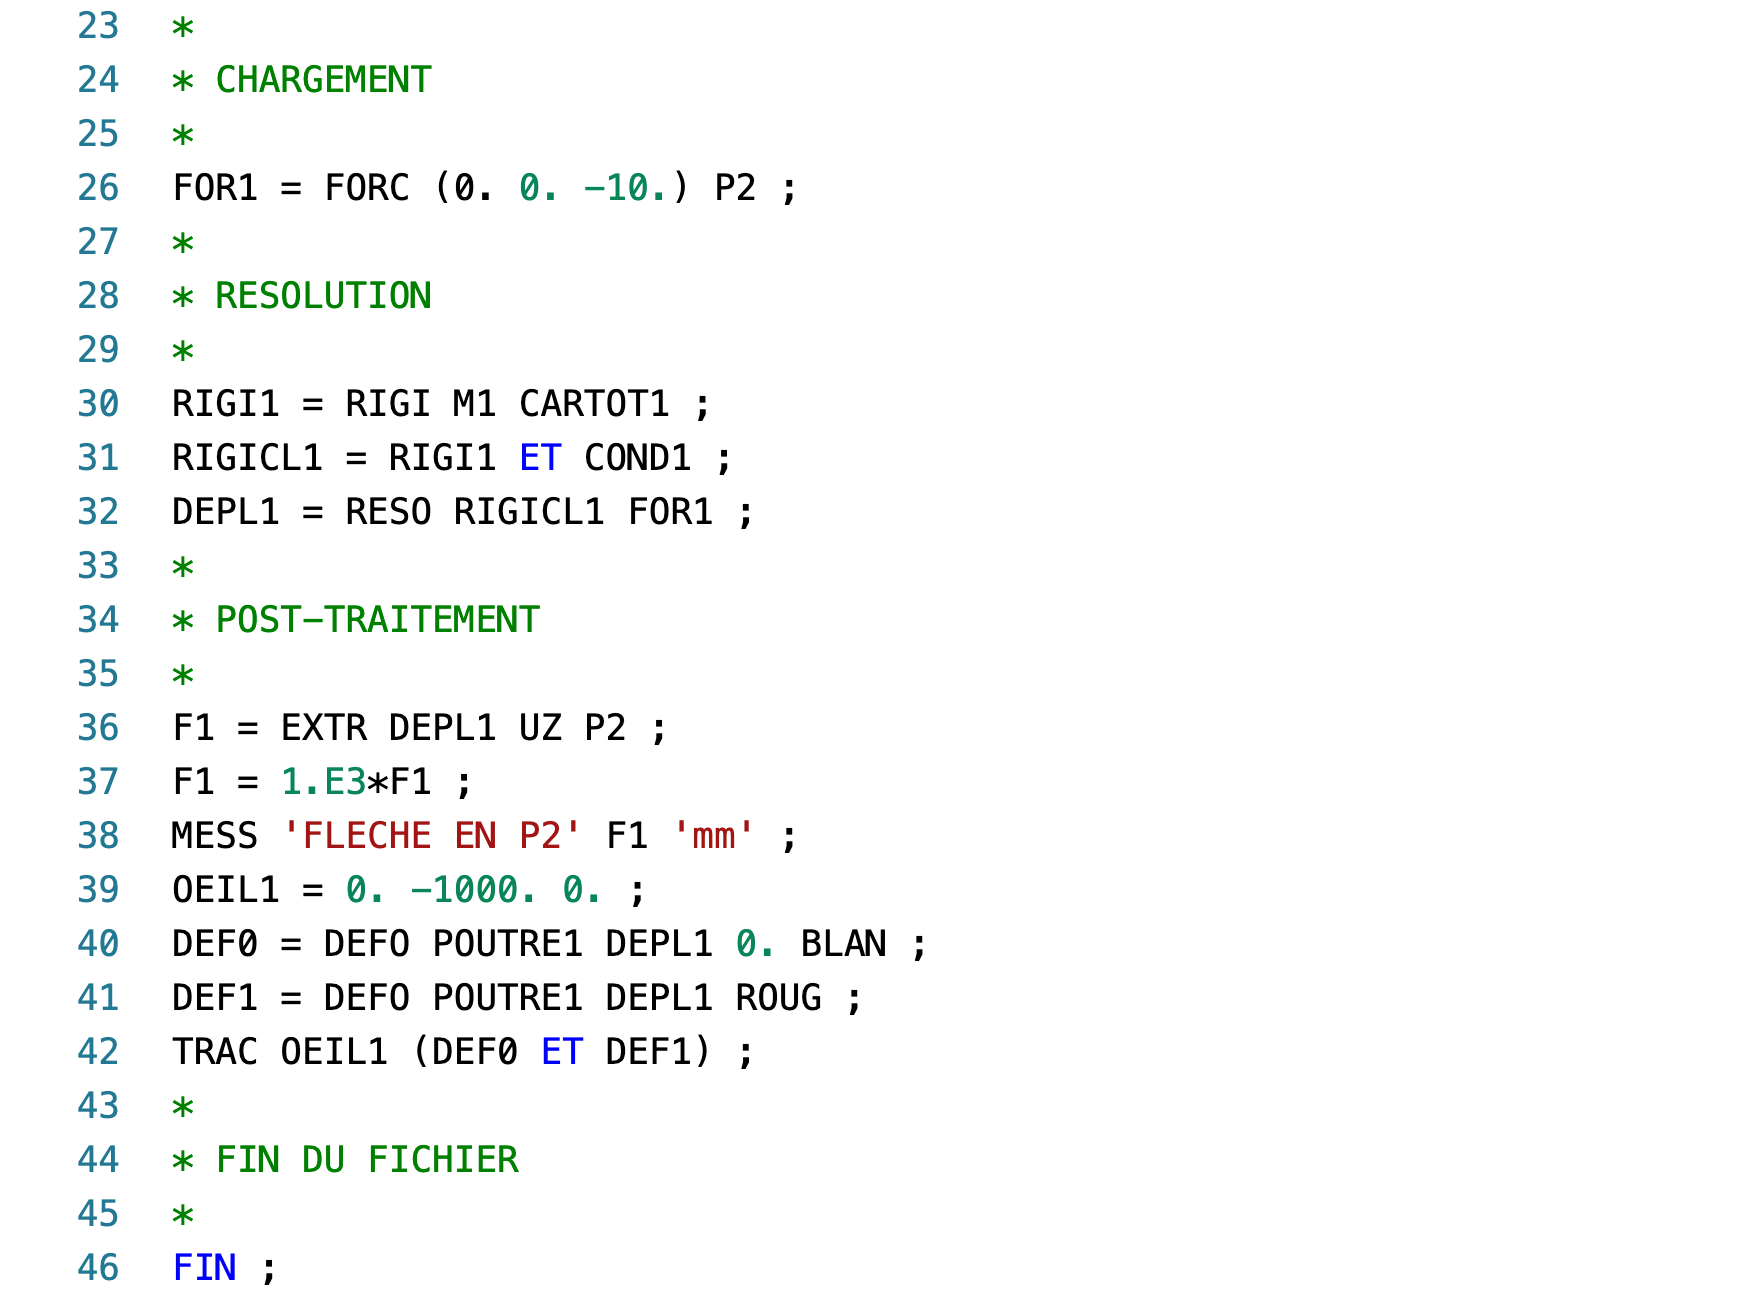
\includegraphics[scale=0.21]{poutre12.png} 
\end{multicols}
Le résultat recherché est la flèche à l'extrémité.

\subsection*{Analyse de la solution}
\subsubsection*{Début de l'étude :}
\begin{verbatim}
TITR 'PREMIER CALCUL MÉCANIQUE' ;  *Donne un nom à l'étude.
OPTI DIME 3 ELEM SEG2 ;
\end{verbatim}
Le problème mécanique nous amène à choisir des éléments finis de type poutre. La documentation nous informe que les éléments géométriques
correspondant à l'élément {\tt POUT} sont des {\tt SEG2} et que la dimension requise pour ce type d'étude est 3.
\subsubsection*{Définition de la géométrie :}
\begin{verbatim}
P1 = 0. 0. 0. ;
P2 = 1. 0. 0. ;
POUTRE1 = P1 DROI 10 P2 ;
\end{verbatim}
La géométrie est décrite en plaçant les points extrémités {\tt P1} et {\tt P2}, et en traçant une ligne droite entre {\tt P1} et {\tt P2} contenant 10 segments.

\subsubsection*{Choix du modèle de comportement et du type d'Eléments Finis :}
\begin{verbatim}
M1=MODE POUTRE1 MECANIQUE ELASTIQUE ISOTROPE POUT ;
\end{verbatim}
L'opérateur {\tt MODE(LE)} sert à définir un type de comportement et une formulation E.F. qui seront affectés à un objet de type maillage. L'objet créé (ici {\tt M1} ) est de type {\tt MMODEL}. On a affecté sur la géométrie {\tt POUTRE1} des éléments finis de type {\tt POUT} et une loi de comportement mécanique élastique isotrope.
\subsubsection*{Entrée des caractéristiques des matériaux et de la MEF} 
\begin{verbatim}
CARMAT1=MATE M1 YOUN 2.E11 NU 0.3 RHO 7.8E3 ;
\end{verbatim}
MATE(RIAU) sert à définir les propriétés physiques du matériau (Module d'Young, coefficient de Poisson...) pour un modèle donné. L'objet créé est de type champ par élément
(MCHAML) à plusieurs composantes : YOUN, NU, RHO, ALPH,...
\begin{verbatim}
CAREF1=CARA M1 SECT....... TORS 1.E10 ;
\end{verbatim}
Certains éléments nécessitent la donnée de caractéristiques supplémentaires qui ne peuvent se déduire de la géométrie. Dans le cas des poutres (POUT) il faut préciser SECT, INRY, INRZ, TORS. Dans le cas des barres (BARR) il suffit de préciser la section. 
\begin{verbatim}
CARTOT1=CARMAT1 ET CAREF1 ;
\end{verbatim}
On prend en compte dans CARTOT1 l'ensemble des caractéristiques définies. On peut préciser ici que tout cela aurait pu s'écrire en une seule ligne :
\begin{verbatim}
CARTOT1=MATE M1 YOUN......TORS 1.E10 ;
\end{verbatim}
Cependant, il nous a semblé pédagogique de séparer les caractéristiques suivant leurs origines. D'autre part, il ne faut pas oublier qu'une ligne d'instructions ne doit comprendre que 72 caractères au maximum.
\subsubsection*{Conditions aux limites} 
\begin{verbatim}
COND1=BLOQ DEPL ROTA P1 ;
\end{verbatim}
Les conditions aux limites sont traitées dans CAST3M comme une rigidité à adjoindre à la rigidité du système libre grâce à l'opérateur {\tt BLOQ(UER)}

\subsubsection*{Conditions de chargement :} 
\begin{verbatim}
FOR1=FORC (0. 0. -10.) P2 ;
\end{verbatim}

Définir le chargement revient à définir un champ par point correspondant au vecteur du second membre de $[K]\{u\} = \{f\}$. Ici on applique une force de $-10$N suivant l'axe $z$ au point {\tt P2}. Ceci s'effectue avec l'opérateur  {\tt FORC(E)}. On aurait pu également écrire
\begin{verbatim}
FOR1=FORC FZ -10. P2 ;
\end{verbatim}
La syntaxe de l'opérateur {\tt MOME(NT)} est du même type. L'opérateur pression, sera quant à lui étudié ultérieurement.


\subsubsection*{Résolution :}
 L'ensemble des données étant défini, on peut constituer le système $[K]\{u\} = \{f\}$ et le résoudre.
 \begin{verbatim}
RIGI1=RIGI M1 CARTOT1 ;
\end{verbatim}
L'opérateur {\tt RIGI(DITE)} permet de construire la matrice de rigidité à partir du modèle et des caractéristiques relatives au modèle.
 \begin{verbatim}
RIGICL1=RIGI1 ET COND1 ;
\end{verbatim}

Comme nous l'avons dit dans le paragraphe conditions aux limites, il convient de prendre en compte la matrice des blocages au sein de la matrice rigidité.
 \begin{verbatim}
DEPL1=RESO RIGICL1 FOR1 ;
\end{verbatim}

L'opérateur {\tt RESO(UT)} résout le système $[K]\{u\} = \{f\}$. Ces déplacements, solutions du problème, sont stockés dans {\tt DEPL1}.

\subsubsection*{Post traitement :}
 \begin{verbatim}
F1=EXTR DEPL1 UZ P2 ;
\end{verbatim}
L'opérateur {\tt EXTR(AIRE)} permet d'extraire une composante d'un ensemble de valeurs. Ici on recherche le déplacement en {\tt UZ} du point {\tt P2} au sein du vecteur solution en déplacement {\tt DEPL1}.
 \begin{verbatim}
F1 = 1.E3 * F1 ;
\end{verbatim}
La résolution par {\tt RESO} donne des résultats en mètres avec notre choix d'unité. Pour l'avoir en mm on le multiplie donc par 1000.
 \begin{verbatim}
MESS ‘FLECHE EN P2' F1 ‘mm' ;
\end{verbatim}
La directive {\tt MESS(AGE)} permet d'afficher un message sur l'unité de sortie.
 \begin{verbatim}
OEIL1 = 0. -1000. 0. ;
\end{verbatim}
On définit ici le point à partir duquel sera vue la structure lors des visualisations. On peut ainsi définir de multiples points de vue.
 \begin{verbatim}
DEF0 = DEFO POUTRE1 DEPL1 0. BLAN;
DEF1 = DEFO POUTRE1 DEPL1 ROUG ;
TRAC OEIL1 (DEF0 ET DEF1) ;
\end{verbatim}
L'opérateur {\tt DEFO(RME)} construit la déformée d'une structure à partir de la géométrie initiale et d'un champs de déplacement. On peut également préciser un certain nombre d'options comme la couleur (ici {\tt BLAN(C)} et {\tt ROUG(E)}), ou le facteur d'amplification pour
rendre les phénomènes plus visibles. Ici on utilise un facteur multiplicatif de 0 sur {\tt DEF0}. Ceci permet de visualiser la structure non déformée en même temps que la déformée finale {\tt DEF1}. Cet artifice est nécessaire car la directive {\tt TRAC(ER)} ne peut être appliquée qu'à des objets de même type. On ne pourrait donc pas avoir : 
 \begin{verbatim}
TRAC OEIL1 (POUTRE1 ET DEF1) 
\end{verbatim}
car l'un est de type maillage et l'autre déformée. On remarque également
l'utilisation du point {\tt OEIL1} pour préciser le point de vue selon lequel on doit effectuer le traçage des déformés.

\subsubsection*{fin du programme }
 \begin{verbatim}
FIN ;
\end{verbatim}
La directive {\tt FIN} permet de quitter {\tt CASTEM}.
\subsection*{Poutre en dim 2 }
{\tiny
\begin{minted}[
mathescape,
framesep=2mm,
baselinestretch=1.2,
%fontsize=\footnotesize,
bgcolor=LightGray,
%linenos
]{bash}
************************************************************************
* Poutre 1D elastique
************************************************************************
*
* fichier poutre1D.dgibi
*
TITR 'Poutre 1D élastique' ;
OPTI DIME 2 ELEM SEG2 ;
*
* Données du problème (Unités : m, Pa)
*
F = -100 ;
L = 1.00 ;
h1 = 0.02 ;
b1 = 0.01 ;
E = 2E11 ;
nu1= 0.3 ;
Izz =(h1**3)*b1/12 ;
S1=b1 * h1;
*
* Solution analytique RdM
*
fana0 =F*(L**3)/(3*E*Izz);
*
* Géométrie
*
P1=0. 0. ;
P2 = L 0. ;
NBelements = 10 ;
Poutre1 = P1 DROI NBelements P2 ;
TRAC Poutre1;
*
* Modèle (Comportement et modélisation EF)
*
mo1=MODE Poutre1 MECANIQUE ELASTIQUE ISOTROPE POUT ;
*
* Données matériau et élément
*
ma1=MATE mo1 YOUN E SECT S1 NU nu1 INRZ IZZ;
*
* Conditions aux limites
*
Cond1 =BLOQ UX UY RZ P1 ;
*
* Chargement
*
Force1=FORC (0. F) P2 ;
*
* Résolution
*
Rigi1=RIGI mo1 ma1 ;
RigiCL1=Rigi1 ET Cond1 ;
Depl1=RESO RigiCL1 Force1 ;
*
* Poste Traitement
*
Fleche1=EXTR Depl1 UY P2 ;

MESS 'Flèche CASTEM : ' Fleche1 'm' ;
MESS 'Flèche analytique : ' fana0 'm' ;
*
Def0=DEFO Poutre1 Depl1 0. BLAN ;
Def1=DEFO Poutre1 Depl1 ROUG ;
TRAC (Def0 ET Def1) ;
*
* Fin du fichier
*
FIN ;
\end{minted}
}
\section*{Exercices}
\subsection*{1. Maillage d'un cube}
  A l'aide d'un éditeur de texte, modifier le fichier maillage-cube.dgibi de façon à construire un parallélépipède de base carré de coté 5m et de hauteur 20m. Essayer d'avoir un maillage régulier (i.e. vraiment cubique !). Sauvegarder le fichier sous un autre nom.

On veut remplacer la commande DALL(ER) par SURF(ACE). Commencez par consulter
la documentation concernant ces commandes.
\begin{enumerate}
\item Définir à l'aide de la commande ET un contour fermé carré.
\item Puis définir la surface carré à l'aide de la commande SURF(ACE) avec l'option 'PLAN(E)'.
\item Essayer les autres options juste pour voir.
\end{enumerate}
\subsection*{2. Maillage d'un cylindre}
 A l'aide des instructions CERC(LE), SURF(ACE) et VOLU(ME) nous allons construire un
cylindre de base circulaire de centre (0, 0, 0) de rayon 2m et hauteur 10m. Pour obtenir la
syntaxe de ces commandes, consulter la documentation en ligne.
\begin{enumerate}
\item Pour commencer, construire 4 quarts de cercle avec la commande CERC(LE).
\item  Réunir les quatres morceaux précédent avec la commande ET.
\item  Utiliser la commande SURF(ACE) avec l'option 'PLAN(E)' pour construire un disque.
\item  Achever la construction du cylindre à l'aide de la commande VOLU(ME).
\item  Construire un cylindre creux de hauteur 10m et dont la base est une couronne délimité
par deux cercles de centre (0, 0, 0) et de rayon respectifs 2m et 2.5m. Indication : tracer
les deux cercles comme précédemment, les réunir à l'aide de la commande ET puis définir
la couronne à l'aide de la commande SURF(ACE). Esayer d'obtenir un maillage régulier.
\end{enumerate}
\subsection*{3. Maillage d'une plaque trouée}
\begin{enumerate}
\item En dimension 2, créer le maillage d'une plaque carré de coté 5m troué d'un disque de
rayon 1m. Indication construire le contour du carré puis du cercle. Les réunir, puis
utiliser ensuite la commande SURF(ACE).
\item  Même chose en dimension 3.
\end{enumerate}

\subsection*{3. Treillis }
Exécuter puis modifier le fichier {\tt barresArticulees.dgibi}  disponible sur e-campus afin d'étudier la structure des barres articulées de TP1. Comparer avec le résultat de TP1.

% Modifier le fichier {\tt poutre.dgibi}  afin d'étudier une poutre droite
%bi-encastrée aux extrémités et soumise à une charge continue de densité linéique constante le long de la poutre ( voir la commande {\tt PRES(SION)}).

 \subsection*{4. Modélisation d'un pont}
 On considère un pont plan de dimensions $L = 20$ mm, $H = 8$ mm et d'épaisseur $e =5$ mm. Son ouverture est en demi cercle central de rayon $R = 5$ m. Ses caractéristiques élastiques sont :
$E = 200$ GP a, $\nu= 0.3$. La charge appliquée est linéique de densité $q = e\times \sigma$ avec 
$\sigma = 500$MP.

\begin{enumerate}
\item On suppose les contraintes et les déformations planes et on choisit d'étudier le pont dans son plan de symétrie verticale et on choisit comme élément fini de référence le triangle de type (1) {\tt TRI3} :
\begin{verbatim}
OPTION DIMENSION 2 ELEMENT TRI3 MODE PLAN CONTRAINTES;
\end{verbatim}
\item  Réaliser un maillage de la plaque avec une densité $\frac{R\pi}{15}$ (équivalent à 15 éléments autour de la partie circulaire):
\begin{verbatim}
DENSITE  R*PI/15;
\end{verbatim}
\item Tracer le maillage avec l'option de calification:
\begin{verbatim}
CONT1=D1 ET D2 ET D3 ET D4 ET D5 ET C1;
SURF1=SURFACE CONT1 PLANE;
TRACER SURF1 QUAL;
\end{verbatim}
\item  Définir le modèle mécanique ainsi que les caractéristiques physiques:
\begin{verbatim}
MOD1=MODELE SURF1 MECANIQUE ELASTIQUE PLASTIQUE PARFAIT;
MAT1=MATE MOD1 YOUN 2.1E11 NU 0.28 DIM3 EP1 SIGY SIGE;
\end{verbatim} 
\item  Appliquer les conditions aux limites en bloquant les déplacements en $x$ et $y$ le long de $D1$ et $D5$ et en imposant une contrainte $\sigma e$ le long de $D3$:
\begin{verbatim}
CL1=BLOQ D1 ..... ; CL2=BLOQ .... .....;
F1=PRESSION MASSIF MOD1 D3 (SIGE*EP1);
\end{verbatim}
\item Définir la rigidité matérielle en appliquant l'opérateur {\tt RIGI} au modèle mécanique {\tt MOD1} en tenant compte des caractéristiques physiques {\tt MAT1}: 
\begin{verbatim}
RIG1 = RIGI ....  ....;
\end{verbatim}
\item Assembler avec les raideurs dues aux conditions aux limites ({\tt CL1} et  {\tt CL2}) avec la rigidité matérielle {\tt RIG1}  pour obtenir la rigidité totale {\tt RITOT}:
\begin{verbatim}
RITOT = .... ET .... ET ....;
\end{verbatim}
\item Résoudre à l'aide de l'opérateur {\tt RESOU}, le système linéaire $K U= F$ où $K$ est la matrice de rigidité totale notée ici {\tt RITOT}, $U$ est le champ de déplacement inconnu noté {\tt DEP1} et $F$ le second membre noté ici {\tt F1}
\begin{verbatim}
DEP1=RESOU ....  .... ;
\end{verbatim}
\item Tracer enfin, l’état de contrainte sur la déformée en faisant:
\begin{verbatim}
DEF1=DEFO DEP1 SURF1;
SIG1=SIGMA DEP1 MOD1 MAT1;
TRACER SIG1 MOD1 DEF1;
\end{verbatim}
\item Refaire la même étude en remplaçant le demi cercle par un rectangle de largeur $2R$ et de hauteur $R$.
\end{enumerate}

\begin{center}
 \begin{tikzpicture}[scale=0.5]
\draw  [very thin, blue] [->]  (-11,0) -- (11,0) node[right] {$x$};
\draw  [very thin, blue] [->]  (0,-1) -- (0,10) node[right] {$y$};

\draw (5,-0.5)--++(5,0) node[midway, below] {$\scriptstyle D_1=5m$};

\draw[olive,<->,dashed] (5,-0.5)--++(5,0) node[midway, below] {$\scriptstyle D_1=5m$};
\draw[olive,<->,dashed] (10.5,0)--++(0,8) node[midway, right] {$\scriptstyle D_2=8m$};
\draw[olive,<->,dashed] (10,7.5)--++(-20,0) node[midway, below] {$\scriptstyle D_3=20m$};
\draw[olive,<->,dashed] (-10.5,8)--++(0,-8) node[midway, left] {$\scriptstyle D_4=8m$};
\draw[olive,<->,dashed] (-10,-0.5)--++(5,0) node[midway, below] {$\scriptstyle D_5=5m$};
\draw[olive,<->,dashed] (-5,-0.5)--++(5,0) node[midway, below] {$\scriptstyle 5m$};
\draw[olive,<->,dashed] (0,-0.5)--++(5,0) node[midway, below] {$\scriptstyle 5m$};


\pgfmathsetmacro{\X}{-10}
\foreach \x in {0,0.1,...,5.1}{
\draw (\X+\x,0) --++ (-0.2,-0.2);
}
\pgfmathsetmacro{\X}{5}
\foreach \x in {0,0.1,...,5.1}{
\draw (\X+\x,0) --++ (-0.2,-0.2);
}

\foreach \x in {-10,-9.5,...,10}{
\draw[very thick,red,latex-] (\x,8)--++(0,1.5);

\draw[gray, line width=1mm, opacity=.5] (5,0) arc[start angle=0, end angle=180, radius=5cm];
}
\draw[gray, line width=1mm, opacity=.5](5,0)--++(5,0)--++(0,8)--++(-20,0)--++(0,-8)--++(5,0);
\end{tikzpicture} 

\end{center}


\end{document}


